%%%%%%%%%%%%%%%%%%%%%%%%%%%%%%%%%%%%%%%%%
% Journal Article
% Distributed Parallel System
% Assignment 2: Ray Framework
%
% Gahan M. Saraiya
% 18MCEC10
%
% References
% ==========
% https://ray.readthedocs.io/en/latest/tutorial.html#overview
% https://ray.readthedocs.io/en/latest/user-profiling.html
% https://towardsdatascience.com/modern-parallel-and-distributed-python-a-quick-tutorial-on-ray-99f8d70369b8
%%%%%%%%%%%%%%%%%%%%%%%%%%%%%%%%%%%%%%%%%
\documentclass[11pt,a4paper,titlepage]{article}
\usepackage[a4paper]{geometry}
\usepackage[utf8]{inputenc}
\usepackage[english]{babel}
\usepackage{lipsum}
%\documentclass[12pt,letterpaper]{article}
%\usepackage{fullpage}
%\usepackage[top=2cm, bottom=4.5cm, left=2.5cm, right=2.5cm]{geometry}
%\usepackage{amsmath,amsthm,amsfonts,amssymb,amscd}
%\usepackage{lastpage}
%\usepackage{enumerate}
%\usepackage{fancyhdr}
%\usepackage{mathrsfs}
%\usepackage{xcolor}
%\usepackage{graphicx}
\usepackage{listings}
\usepackage{minted}
%\usepackage{hyperref}
%\usepackage{longtable}

\usepackage{amsmath, amssymb, amsfonts, amsthm, fouriernc, mathtools}
% mathtools for: Aboxed (put box on last equation in align envirenment)
\usepackage{microtype} %improves the spacing between words and letters

\usepackage{graphicx}
\graphicspath{ {./assets/} {./pics/} {./eps/}}
\usepackage{epsfig}
\usepackage{epstopdf}


%%%%%%%%%%%%%%%%%%%%%%%%%%%%%%%%%%%%%%%%%%%%%%%%%%
%% COLOR DEFINITIONS
%%%%%%%%%%%%%%%%%%%%%%%%%%%%%%%%%%%%%%%%%%%%%%%%%%
\usepackage[svgnames]{xcolor} % Enabling mixing colors and color's call by 'svgnames'
%%%%%%%%%%%%%%%%%%%%%%%%%%%%%%%%%%%%%%%%%%%%%%%%%%
\definecolor{MyColor1}{rgb}{0.2,0.4,0.6} %mix personal color
\newcommand{\textb}{\color{Black} \usefont{OT1}{lmss}{m}{n}}
\newcommand{\blue}{\color{MyColor1} \usefont{OT1}{lmss}{m}{n}}
\newcommand{\blueb}{\color{MyColor1} \usefont{OT1}{lmss}{b}{n}}
\newcommand{\red}{\color{LightCoral} \usefont{OT1}{lmss}{m}{n}}
\newcommand{\green}{\color{Turquoise} \usefont{OT1}{lmss}{m}{n}}
%%%%%%%%%%%%%%%%%%%%%%%%%%%%%%%%%%%%%%%%%%%%%%%%%%




%%%%%%%%%%%%%%%%%%%%%%%%%%%%%%%%%%%%%%%%%%%%%%%%%%
%% FONTS AND COLORS
%%%%%%%%%%%%%%%%%%%%%%%%%%%%%%%%%%%%%%%%%%%%%%%%%%
%    SECTIONS
%%%%%%%%%%%%%%%%%%%%%%%%%%%%%%%%%%%%%%%%%%%%%%%%%%
\usepackage{titlesec}
\usepackage{sectsty}
%%%%%%%%%%%%%%%%%%%%%%%%
%set section/subsections HEADINGS font and color
\sectionfont{\color{MyColor1}}  % sets colour of sections
\subsectionfont{\color{MyColor1}}  % sets colour of sections

%set section enumerator to arabic number (see footnotes markings alternatives)
\renewcommand\thesection{\arabic{section}.} %define sections numbering
\renewcommand\thesubsection{\thesection\arabic{subsection}} %subsec.num.

%define new section style
\newcommand{\mysection}{
    \titleformat{\section} [runin] {\usefont{OT1}{lmss}{b}{n}\color{MyColor1}} 
    {\thesection} {3pt} {} } 


%Importing csv as table
\usepackage{csvsimple}

\usepackage{longtable}
\renewcommand\thesection{\Roman{section}} % Roman numerals for the sections
\renewcommand\thesubsection{\Roman{subsection}} % Roman numerals for subsections
%----------------------------------------------------------------------------------------
%       DATE FORMAT
%----------------------------------------------------------------------------------------
\usepackage{datetime}
\newdateformat{monthyeardate}{\monthname[\THEMONTH], \THEYEAR}
%----------------------------------------------------------------------------------------

\titleformat{\section}[block]{\large\scshape\centering}{\thesection.}{1em}{} % Change the look of the section titles
\titleformat{\subsection}[block]{\large}{\thesubsection.}{1em}{} % Change the look of the section titles
\newcommand{\horrule}[1]{\rule{\linewidth}{#1}} % Create horizontal rule command with 1 argument of height
\usepackage{fancyhdr} % Headers and footers
\pagestyle{fancy} % All pages have headers and footers
\fancyhead{} % Blank out the default header
\fancyfoot{} % Blank out the default footer



%%%%%%%%%%%%%%%%%%%%%%%%%%%%%%%%%%%%%%%%%%%%%%%%%%
%		CAPTIONS
%%%%%%%%%%%%%%%%%%%%%%%%%%%%%%%%%%%%%%%%%%%%%%%%%%
\usepackage{caption}
\usepackage{subcaption}
%%%%%%%%%%%%%%%%%%%%%%%%
\captionsetup[figure]{labelfont={color=Turquoise}}

%%%%%%%%%%%%%%%%%%%%%%%%%%%%%%%%%%%%%%%%%%%%%%%%%%
%		!!!EQUATION (ARRAY) --> USING ALIGN INSTEAD
%%%%%%%%%%%%%%%%%%%%%%%%%%%%%%%%%%%%%%%%%%%%%%%%%%
%using amsmath package to redefine eq. numeration (1.1, 1.2, ...) 
%%%%%%%%%%%%%%%%%%%%%%%%
\renewcommand{\theequation}{\thesection\arabic{equation}}

%set box background to grey in align environment 
\usepackage{etoolbox}% http://ctan.org/pkg/etoolbox
\makeatletter
\patchcmd{\@Aboxed}{\boxed{#1#2}}{\colorbox{black!15}{$#1#2$}}{}{}%
\patchcmd{\@boxed}{\boxed{#1#2}}{\colorbox{black!15}{$#1#2$}}{}{}%
\makeatother
%%%%%%%%%%%%%%%%%%%%%%%%%%%%%%%%%%%%%%%%%%%%%%%%%%




%%%%%%%%%%%%%%%%%%%%%%%%%%%%%%%%%%%%%%%%%%%%%%%%%%
%% DESIGN CIRCUITS
%%%%%%%%%%%%%%%%%%%%%%%%%%%%%%%%%%%%%%%%%%%%%%%%%%
\usepackage[siunitx, american, smartlabels, cute inductors, europeanvoltages]{circuitikz}
%%%%%%%%%%%%%%%%%%%%%%%%%%%%%%%%%%%%%%%%%%%%%%%%%%



\makeatletter
\let\reftagform@=\tagform@
\def\tagform@#1{\maketag@@@{(\ignorespaces\textcolor{red}{#1}\unskip\@@italiccorr)}}
\renewcommand{\eqref}[1]{\textup{\reftagform@{\ref{#1}}}}
\makeatother
\usepackage{hyperref}
\hypersetup{colorlinks=true}

\usepackage{makecell}
\hypersetup{%
  colorlinks=true,
  linkcolor=blue,
  linkbordercolor={0 0 1}
}
 
\renewcommand\lstlistingname{Algorithm}
\renewcommand\lstlistlistingname{Algorithms}
\def\lstlistingautorefname{Alg.}

\lstdefinestyle{Python}{
    language        = Python,
    frame           = lines, 
    basicstyle      = \footnotesize,
    keywordstyle    = \color{blue},
    stringstyle     = \color{green},
    commentstyle    = \color{red}\ttfamily
}

\setlength{\parindent}{0.0in}
\setlength{\parskip}{0.05in}

%% Edit these as appropriate
%% \newcommand\course{CSE 3500}
%\newcommand\hwnumber{1}                  % <-- homework number
%\newcommand\NetIDa{Gahan M. Saraiya}           % <-- NetID of person #1
%\newcommand\NetIDb{18MCEC10}           % <-- NetID of person #2 (Comment this line out for problem sets)
%
%\pagestyle{fancyplain}
%\headheight 35pt
%\lhead{\NetIDa}
%\lhead{\NetIDa\\\NetIDb}                 % <-- Comment this line out for problem sets (make sure you are person #1)
%\chead{\textbf{\Large DPS Assignment \hwnumber}}
%\rhead{\course \\ \today}
%\lfoot{}
%\cfoot{}
%\rfoot{\small\thepage}
%\headsep 1.5em
%%%%%%%%%%%%%%%%%%%%%%%%%%%%%%%%%%%%%%%%%%%%%%%%%%
%% PREPARE TITLE
%%%%%%%%%%%%%%%%%%%%%%%%%%%%%%%%%%%%%%%%%%%%%%%%%%
\title{\blue Distributed Parallel System \\
    \blueb Assignment $2$ - Ray Framework}
\author{Gahan Saraiya (18MCEC10)}
\date{\monthyeardate\today}
%\date{March, 2019}
%%%%%%%%%%%%%%%%%%%%%%%%%%%%%%%%%%%%%%%%%%%%%%%%%%
%----------------------------------------------------------------------------------------
%       SET HEADER AND FOOTER
%----------------------------------------------------------------------------------------
\newcommand\theauthor{Gahan Saraiya}
\newcommand\thesubject{Distributed Parallel System}
\renewcommand{\footrulewidth}{0.4pt}% default is 0pt
\fancyhead[C]{Institute of Technology, Nirma University $\bullet$ \monthyeardate\today} % Custom header text
\fancyfoot[LE,LO]{\thesubject}
\fancyfoot[RO,LE]{Page \thepage} % Custom footer text
%----------------------------------------------------------------------------------------

\usepackage[utf8]{inputenc}
\usepackage[english]{babel}
\usepackage[utf8]{inputenc}
\usepackage{fourier} 
\usepackage{array}
\usepackage{makecell}

\renewcommand\theadalign{bc}
\renewcommand\theadfont{\bfseries}
\renewcommand\theadgape{\Gape[4pt]}
\renewcommand\cellgape{\Gape[4pt]}
\newcommand*\tick{\item[\Checkmark]}
\newcommand*\arrow{\item[$\Rightarrow$]}
\newcommand*\fail{\item[\XSolidBrush]}
\usepackage{minted} % for highlighting code sytax
\definecolor{LightGray}{gray}{0.9}
\renewcommand*{\arraystretch}{2}
%\definecolor{LightGray}{gray}{0.9}

\setminted[text]{
	frame=lines, 
	breaklines,
	baselinestretch=1.2,
	bgcolor=LightGray,
%	fontsize=\small
}
\setminted[bash]{
%	frame=lines, 
	breaklines,
	baselinestretch=1.2,
	bgcolor=LightGray,
%	fontsize=\small
}
\setminted[python]{
	frame=lines, 
	breaklines, 
	linenos,
	baselinestretch=1.2,
%	bgcolor=LightGray,
%	fontsize=\small
}


\begin{document}
\maketitle

\section{Introduction}
Parallel and distributed computing are a staple of modern applications. We need to leverage multiple cores or multiple machines to speed up applications or to run them at a large scale. The infrastructure for crawling the web and responding to search queries are not single-threaded programs running on someone’s laptop but rather collections of services that communicate and interact with one another.

The cloud promises unlimited scalability in all directions (memory, compute, storage, etc). Realizing this promise requires new tools for programming the cloud and building distributed applications.

\begin{figure}[!htbp]
    \centering
    
\includegraphics[width=\textwidth]{ray-logo}
\end{figure}

To task advantage of this unlimited scalability this experiment aims towards building application with Ray Framework build in python which can scale from \verb|laptop to large cluster|.


\subsection{Significance of Ray}
Ray is capable to handle requirements of modern days application listed below:
\begin{itemize}
    \item Running the same code on more than one machine.
    \item Building micro-services and actors that have state and can communicate.
    \item Gracefully handling machine failures.
    \item Efficiently handling large objects and numerical data.
\end{itemize}

Traditional Programming rely on 2 core concepts:
\begin{itemize}
    \item functions
    \item classes
\end{itemize}
Using these building blocks, programming languages allow us to build countless applications.

However, when we migrate our applications to the distributed setting, the concepts typically change.

On one end of the spectrum, we have tools like \href{https://www.open-mpi.org/}{OpenMPI}, \verb|Python multiprocessing|, and \href{http://zeromq.org/}{ZeroMQ}, which provide low-level primitives for sending and receiving messages. These tools are very powerful, but they provide a different abstraction and so single-threaded applications must be rewritten from scratch to use them.

On the other end of the spectrum, we have domain-specific tools like \href{https://www.tensorflow.org/}{TensorFlow} for model training, \href{https://spark.apache.org/}{Spark} for data processing and SQL, and \href{https://flink.apache.org/}{Flink} for stream processing. These tools provide higher-level abstractions like neural networks, datasets, and streams. However, because they differ from the abstractions used for serial programming, applications again must be rewritten from scratch to leverage them.

\begin{figure}[!htbp]
    \centering
    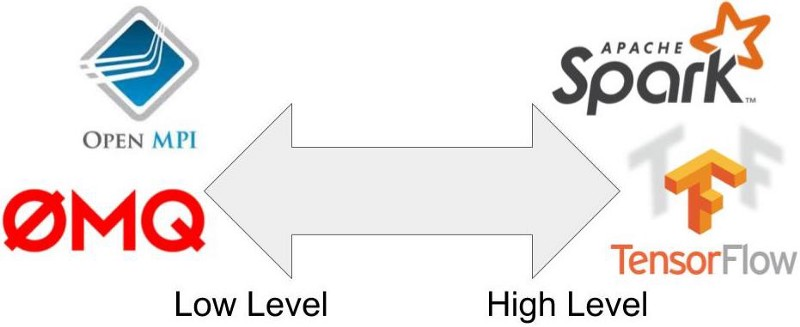
\includegraphics[width=0.7\textwidth]{distributed-computing-app}
    \caption{Tools for distributed computing on an axis from low-level primitives to high-level abstractions.}
\end{figure}

Ray occupies a unique middle ground. Instead of introducing new concepts. Ray takes the existing concepts of functions and classes and translates them to the distributed setting as tasks and actors. This API choice allows serial applications to be parallelized without major modifications.

\section{Introduction to Ray}
Ray is a distributed execution engine. The same code can be run on a single machine to achieve efficient multiprocessing, and it can be used on a cluster for large computations.

When using Ray, several processes are involved.

\begin{itemize}
    \item Multiple worker processes execute tasks and store results in object stores. Each worker is a separate process.
    \item One object store per node stores immutable objects in shared memory and allows workers to efficiently share objects on the same node with minimal copying and deserialization.
    \item One raylet per node assigns tasks to workers on the same node.
    \item A driver is the Python process that the user controls. For example, if the user is running a script or using a Python shell, then the driver is the Python process that runs the script or the shell. A driver is similar to a worker in that it can submit tasks to its raylet and get objects from the object store, but it is different in that the raylet will not assign tasks to the driver to be executed.
    \item A Redis server maintains much of the system’s state. For example, it keeps track of which objects live on which machines and of the task specifications (but not data). It can also be queried directly for debugging purposes.
\end{itemize}

\subsection{Initializing Ray}
To start Ray, start Python and run the following commands:
\begin{minted}{python}
import ray
ray.init()
\end{minted}

The \verb|ray.init()| command starts all of the relevant Ray processes. 

On a cluster, this is the only line that needs to change (we need to pass in the cluster address). These processes include the following:
\begin{itemize}
    \item A number of worker processes for executing Python functions in parallel (roughly one worker per CPU core).
    \item A scheduler process for assigning “tasks” to workers (and to other machines). A task is the unit of work scheduled by Ray and corresponds to one function invocation or method invocation.
    \item A shared-memory object store for sharing objects efficiently between workers (without creating copies).
    \item An in-memory database for storing metadata needed to rerun tasks in the event of machine failures.
\end{itemize}

Ray workers are separate processes as opposed to threads because support for multi-threading in Python is very limited due to the \href{https://wiki.python.org/moin/GlobalInterpreterLock}{global interpreter lock}.

\subsection{Asynchronous Computation in Ray}
Ray enables arbitrary Python functions to be executed asynchronously. This is done by designating a Python function as a remote function.

For example, a normal Python function looks like below:
\begin{minted}{python}
def add1(a, b):
    return a + b
\end{minted}

A remote function looks like this.
\begin{minted}{python}
@ray.remote
def add2(a, b):
    return a + b
\end{minted}

Whereas calling \verb|add1(1, 2)| returns \verb|3| and causes the Python interpreter to block until the computation has finished, calling \verb|add2.remote(1, 2)| immediately returns an object ID and creates a task. The task will be scheduled by the system and executed asynchronously (potentially on a different machine). When the task finishes executing, its return value will be stored in the object store.

The following simple example demonstrates how asynchronous tasks can be used to parallelize computation:

\begin{minted}{python}
import time

def foo():
    time.sleep(1)

@ray.remote
def bar():
    time.sleep(1)

# The following takes ten seconds.
[foo() for _ in range(10)]

# The following takes one second (assuming the system has at least ten CPUs).
ray.get([bar.remote() for _ in range(10)])
\end{minted}

There is a sharp distinction between submitting a task and executing the task. When a remote function is called, the task of executing that function is submitted to a raylet, and object IDs for the outputs of the task are immediately returned. However, the task will not be executed until the system actually schedules the task on a worker. Task execution is not done lazily. The system moves the input data to the task, and the task will execute as soon as its input dependencies are available and there are enough resources for the computation.

When a task is submitted, each argument may be passed in by value or by object ID. For example, these lines have the same behavior.

\begin{minted}{python}
add2.remote(1, 2)
add2.remote(1, ray.put(2))
add2.remote(ray.put(1), ray.put(2))
\end{minted}

\section{Parallelism with Tasks}
To turn a Python function \verb|foo| into a “remote function” (a function that can be executed remotely and asynchronously), we declare the function with the \verb|@ray.remote| decorator. Then function invocations via \verb|f.remote()| will immediately return futures (a future is a reference to the eventual output), and the actual function execution will take place in the background (we refer to this execution as a task).

\inputminted{python}{../src/01.TaskParallelism.py}

Because the call to \verb|foo.remote(i)| returns immediately, four copies of \verb|foo| can be executed in parallel simply by running that line four times.

\subsection{Task Dependencies}
Tasks can also depend on other tasks. Below, the \verb|multiply_matrices| task uses the outputs of the two \verb|create_matrix| tasks, so it will not begin executing until after the first two tasks have executed. The outputs of the first two tasks will automatically be passed as arguments into the third task and the futures will be replaced with their corresponding values). In this manner, tasks can be composed together with arbitrary DAG dependencies.

\subsection{Aggregating Values Efficiently}
Task dependencies can be used in much more sophisticated ways. For example, suppose we wish to aggregate 8 values together. This example uses integer addition, but in many applications, aggregating large vectors across multiple machines can be a bottleneck. In this case, changing a single line of code can change the aggregation’s running time from linear to logarithmic in the number of values being aggregated.

\begin{figure}[!htbp]
    \centering
    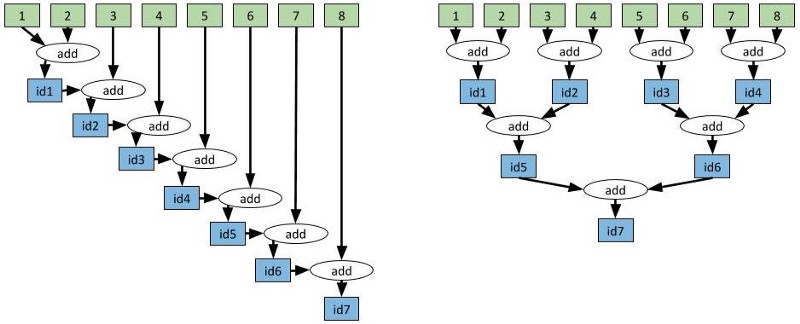
\includegraphics[width=\textwidth]{aggregating-values}
    \caption{The dependency graph on the left has depth 7. The dependency graph on the right has depth 3. The computations yield the same result, but the one on the right is much faster.}
\end{figure}

As described above, to feed the output of one task as an input into a subsequent task, simply pass the future returned by the first task as an argument into the second task. This task dependency will automatically be taken into account by Ray’s scheduler. The second task will not execute until the first task has finished, and the output of the first task will automatically be shipped to the machine on which the second task is executing.

\inputminted{python}{../src/03.ExplicitAggregation.py}

The above code is very explicit, but note that both approaches can be implemented in a more concise fashion using while loops.


\inputminted{python}{../src/04.aggregationConciese.py}

\section{From Classes to Actors}
It’s challenging to write interesting applications without using classes, and this is as true in the distributed setting as it is on a single core.

Ray allows you to take a Python class and declare it with the @ray.remote decorator. Whenever the class is instantiated, Ray creates a new “actor”, which is a process that runs somewhere in the cluster and holds a copy of the object. Method invocations on that actor turn into tasks that run on the actor process and can access and mutate the state of the actor. In this manner, actors allow mutable state to be shared between multiple tasks in a way that remote functions do not.

Individual actors execute methods serially (each individual method is atomic) so there are no race conditions. Parallelism can be achieved by creating multiple actors.

%\inputminted{python}{../src/05.ActorsClasses}

    The above example is the simplest possible usage of actors. The line \verb|Counter.remote()| creates a new actor process, which has a copy of the Counter object. The calls to c.\verb|get_value.remote|() and c.inc.remote() execute tasks on the remote actor process and mutate the state of the actor.
\section{Tuning and profiling}\label{section:proifiling}
For the profiling I have implemented a simple code of $ O(n^2) $ as shown below:
\begin{minted}{python}
sum([i*j*1 
    for i in range(n) 
    for j in range(n) 
    for k in range(1)
])
\end{minted}
As you can see the code will compute multiplication of every permutation of $ n $ (integer number provided for computation) and then calculating sum of all these numbers.

\subsection{Sequential Code}\label{subsec:sequential}
\inputminted{python}{../src/experiment.py}\label{code:seq}

\subsubsection{Output}
\inputminted{text}{../src/outputNonRay.txt}


\subsection{Parallel Code}\label{subsec:parallel}
Below is the implementation of parallel code with single node and 4 cores: 
\inputminted{python}{../src/experimentRay.py}\label{code:parallel}

\subsubsection{Output}
\inputminted{text}{../src/outputRay.txt}


\section{Summarizing Performance}
As you can see in the code implemented in section \ref{section:proifiling}.\ref{subsec:sequential}.\ref{code:seq} is sequential and the amount of time (in seconds) is increased by the number of iterations.

\begin{table}[H]
    \centering
    \renewcommand{\arraystretch}{1.5}
    \begin{tabular}{| l | p{4cm} | p{4cm} |}%
        \hline
        \bfseries Number of Data ($ n $)
        & \bfseries Sequential code [\ref{section:proifiling}.\ref{subsec:sequential}.\ref{code:seq}] execution (in seconds)
        & \bfseries Parallel code [\ref{section:proifiling}.\ref{subsec:parallel}.\ref{code:parallel}] execution (in seconds) (with \textit{1 node and 4 cores}) 
        \csvreader{../src/observation.csv}{}% use head of csv as column names
        {
            \\ \hline
            \csvcoli 
            &\csvcolii
            &\csvcoliii
        }
        \\ \hline
    \end{tabular}
    
    \caption{result of observation (Note that due to limitation of resources the code can not be executed with more than one nodes)}\label{table:observations}
%    \medskip
%    \small
%    \begin{itemize}
%        \item Here chunk size $ -1 $ represents that no chunk size specified in command 
%        \item $ 100 $ is specified as number of fixed chunk
%        \item $ 250000 $ is the value derived by $ \frac{\text{size of array}}{\text{number of threads}} $
%    \end{itemize}
\end{table}

As observed in result (refer Table \ref{table:observations}) for small data chunk size the overhead observed with Ray implementation, however as data size increases, gradually speedup observed is increased and the parallel version is able to complete the same task can be completed lot quicker.


Various other Tuning implementation with Ray are available at \url{https://github.com/gahan9/ray/tree/master/python/ray/tune/examples}.


\end{document}
